\chapter{DBSCAN, Isolation Forest e Anomaly Detection}
\begin{flushright}\small\textit{Lezione 9 -- 14/04/2026 -- G\'eron, Cap.\ 9 (cont.)}\end{flushright}

\section{DBSCAN: clustering basato sulla densità}

A differenza del K-Means, che si basa sulle distanze dai centroidi, il \textbf{DBSCAN} (\emph{Density-Based Spatial Clustering of Applications with Noise}, Ester et al.\ 1996) definisce i cluster come \textbf{regioni ad alta densità separate da zone a bassa densità}. Non richiede di specificare $k$ a priori.

\subsection{Concetti chiave}

Due iperparametri controllano tutto:
\begin{itemize}
    \item $\boldsymbol{\varepsilon}$ (\emph{epsilon}): raggio del vicinato -- la distanza massima entro cui un punto è considerato ``vicino''.
    \item \texttt{min\_samples}: numero minimo di punti che devono cadere entro $\varepsilon$ perché un punto sia considerato ``denso''.
\end{itemize}

Ogni punto riceve una delle tre etichette:

\begin{center}
\renewcommand{\arraystretch}{1.3}
\begin{tabular}{@{} l p{10cm} @{}}
\toprule
\textbf{Tipo} & \textbf{Definizione} \\
\midrule
\textbf{Core Instance} & Ha almeno \texttt{min\_samples} punti nel raggio $\varepsilon$. È nel cuore di una regione densa. \\
\textbf{Border Point} & Non è core, ma cade entro $\varepsilon$ di una core instance. È ai margini del cluster. \\
\textbf{Noise / Outlier} & Non è core e non è raggiungibile da nessuna core. Etichettato $-1$ in Scikit-learn. \\
\bottomrule
\end{tabular}
\end{center}

\subsection{Funzionamento dell'algoritmo}

\begin{enumerate}
    \item Per ogni punto $x$, contare i vicini nel vicinato $B(x, \varepsilon)$.
    \item Se il conteggio $\geq$ \texttt{min\_samples}, marcare $x$ come \emph{core instance}.
    \item Espandere il cluster: partendo da una core instance, aggiungere tutti i punti \emph{density-reachable} (raggiungibili attraverso una catena di core instances connesse).
    \item I punti non raggiungibili da nessuna core instance sono \emph{noise} -- etichettati $-1$.
\end{enumerate}

\begin{exbox}[Effetto di $\varepsilon$ su make\_moons]
Con $\varepsilon = 0{,}05$ (troppo piccolo): l'algoritmo trova 7 cluster separati e molte anomalie -- troppo restrittivo.

Con $\varepsilon = 0{,}2$ (giusto): trova esattamente 2 cluster (le due mezze lune) con pochissimi punti di rumore -- perfetto per forme non lineari dove K-Means fallisce completamente.
\end{exbox}

\subsection{Vantaggi e limiti}

\begin{itemize}
    \item \textbf{Pro}: cluster di qualsiasi forma (mezze lune, spirali, L-shape); gestisce nativamente il rumore (outlier $= -1$); non richiede di specificare $k$.
    \item \textbf{Contro}: fatica con densità molto variabili tra cluster; scala male in alta dimensione (\emph{curse of dimensionality}); $\varepsilon$ e \texttt{min\_samples} vanno scelti con cura.
\end{itemize}

\begin{notebox}[DBSCAN non ha \texttt{predict()}]
Scikit-learn non fornisce un metodo \texttt{predict()} nativo per DBSCAN. Per classificare nuovi punti, si addestra un classificatore secondario (tipicamente K-NN) sulle core instances. Con una soglia di distanza si può anche rifiutare punti molto lontani come anomalie.

\textbf{HDBSCAN} (Hierarchical DBSCAN): variante che gestisce densità variabili costruendo una gerarchia di cluster -- generalmente superiore a DBSCAN e disponibile nel pacchetto \texttt{scikit-learn-contrib}.
\end{notebox}

\section{Cenno: Gaussian Mixture Models (GMM)}

Il \textbf{Gaussian Mixture Model} è un modello probabilistico che assume che i dati siano stati generati da una miscela di $k$ distribuzioni Gaussiane, ciascuna con il proprio centro $\boldsymbol{\mu}_j$ e la propria forma $\boldsymbol{\Sigma}_j$. A differenza del K-Means, il GMM assegna a ogni istanza una \textbf{probabilità di appartenenza} a ciascun cluster (\emph{soft clustering}) e gestisce cluster di forma ellittica. I parametri si stimano con l'algoritmo EM (Expectation-Maximization). Per scegliere il numero di componenti si usano i criteri AIC e BIC. Il GMM è anche un \textbf{modello generativo}: può campionare nuovi dati dalla distribuzione appresa ed è usato per anomaly detection individuando istanze in regioni a bassa densità.

\section{Isolation Forest: rilevazione delle anomalie}

\textbf{Isolation Forest} (Liu, Ting \& Zhou 2008) è un algoritmo specifico per l'\emph{anomaly detection}, basato sul principio che le \textbf{anomalie sono poche e diverse}: sono più facili da isolare rispetto ai punti normali.

\subsection{Logica fondamentale}

Invece di stimare densità o distanze, Isolation Forest misura \textbf{quanto rapidamente un punto viene isolato} da tagli casuali dello spazio delle feature.

\begin{itemize}
    \item Un \textbf{punto normale} si trova in una regione densa $\to$ servono \emph{molti} tagli casuali per isolarlo $\to$ si trova in foglie profonde dell'albero.
    \item Un'\textbf{anomalia} è lontana dalla massa dei dati $\to$ bastano \emph{pochi} tagli $\to$ si trova vicino alla radice.
\end{itemize}

\begin{center}
\begin{tikzpicture}[font=\small]
\begin{groupplot}[
    group style={group size=2 by 1, horizontal sep=2cm},
    width=5.5cm, height=4.5cm,
    xmin=-4, xmax=4, ymin=-4, ymax=4,
    xtick=\empty, ytick=\empty,
    grid=none,
    title style={font=\small\bfseries}
]
\nextgroupplot[title={Punto normale -- isolato tardi}]
\addplot[only marks, mark=*, mark size=1.5pt, MidnightBlue!60]
    coordinates {(-1,0.5)(-0.5,1)(0,0)(0.5,-0.5)(1,0.8)(-0.8,-0.3)
                 (0.3,0.6)(-0.2,-0.8)(0.7,0.2)(-0.6,0.9)(0.2,-0.3)
                 (-0.9,0.1)(0.5,0.5)(-0.3,0.7)(0.8,-0.6)};
\addplot[only marks, mark=*, mark size=4pt, OliveGreen]
    coordinates {(0.1, 0.2)};
\node[font=\scriptsize, OliveGreen] at (axis cs:0.5, -1.5) {target};
\draw[BrickRed, thick] (axis cs:-4, 0.5) -- (axis cs:4, 0.5);
\draw[BrickRed!60, thick] (axis cs:-1.5, -4) -- (axis cs:-1.5, 0.5);
\node[font=\tiny, BrickRed] at (axis cs:-3, -2) {taglio 1};
\node[font=\tiny, BrickRed!60] at (axis cs:-2.5, 2) {taglio 2};
\node[font=\tiny] at (axis cs:2, 3) {taglio 3 \ldots};
\nextgroupplot[title={Anomalia -- isolata subito}]
\addplot[only marks, mark=*, mark size=1.5pt, MidnightBlue!60]
    coordinates {(-1,0.5)(-0.5,1)(0,0)(0.5,-0.5)(1,0.8)(-0.8,-0.3)
                 (0.3,0.6)(-0.2,-0.8)(0.7,0.2)(-0.6,0.9)(0.2,-0.3)
                 (-0.9,0.1)(0.5,0.5)(-0.3,0.7)(0.8,-0.6)};
\addplot[only marks, mark=triangle*, mark size=4pt, BrickRed]
    coordinates {(3.5, 3.5)};
\node[font=\scriptsize, BrickRed] at (axis cs:3.0, 2.5) {anomalia};
\draw[BrickRed, thick] (axis cs:2, -4) -- (axis cs:2, 4);
\node[font=\tiny, BrickRed] at (axis cs:0.5, -3) {taglio 1: isolata!};
\end{groupplot}
\end{tikzpicture}
\end{center}

\subsection{Come funziona}

\begin{enumerate}
    \item Si costruisce una foresta di \textbf{isolation trees}: ogni albero seleziona una feature a caso, poi una soglia di taglio casuale tra il minimo e il massimo di quella feature nel nodo corrente. Si ricorre finché ogni punto è isolato.
    \item Per ogni punto si calcola la \textbf{lunghezza media del percorso} su tutti gli alberi.
    \item La lunghezza media viene \textbf{normalizzata} rispetto alla lunghezza attesa per un dataset casuale della stessa dimensione.
    \item \textbf{Anomaly score}: più corto è il percorso medio, più anomalo è il punto.
\end{enumerate}

\subsection{Parametri fondamentali}

\begin{itemize}
    \item \texttt{n\_estimators}: numero di alberi nella foresta (default: 100). Più alberi $\to$ meno varianza, ma più lento.
    \item \texttt{contamination}: proporzione attesa di anomalie nel dataset. Controlla direttamente la soglia di classificazione. Impostarlo è una \textbf{decisione di business}: quante anomalie mi aspetto? (es.\ \texttt{0.01} per 1\% di frodi).
    \item \texttt{max\_samples}: numero di istanze per albero (default: \texttt{'auto'} $= \min(256, m)$). Sottocampionare aumenta la diversità tra alberi.
    \item \texttt{max\_features}: numero di feature per albero; ridurlo aumenta la diversità.
\end{itemize}

\subsection{Vantaggi e limiti}

\begin{itemize}
    \item \textbf{Vantaggi}: non calcola distanze né densità $\to$ computazionalmente efficiente; scala bene in alta dimensione; ottimo come baseline per anomaly detection.
    \item \textbf{Limiti}: fallisce se le anomalie formano cluster densi tra loro; i punteggi sono relativi alla distribuzione osservata; sensibile a feature irrilevanti.
\end{itemize}

\begin{notebox}[Outlier detection vs.\ Novelty detection]
\textbf{Outlier detection}: il training set può già contenere anomalie -- il modello le cerca durante il training. È il caso tipico di Isolation Forest.

\textbf{Novelty detection}: il modello è addestrato su dati ``puliti'' (solo normali) e poi usato per rifiutare nuove osservazioni anomale. One-Class SVM è progettato per questo scenario.
\end{notebox}

\section{Analisi esplorativa (EDA) e outlier}

Prima di applicare qualsiasi modello di clustering o anomaly detection, è fondamentale capire la distribuzione dei dati tramite strumenti grafici.

\subsection{Istogrammi e il fenomeno del Capping}

Analizzando gli attributi numerici di un dataset (es.\ dati immobiliari) si possono notare anomalie visive negli istogrammi:

\begin{itemize}
    \item \textbf{Distribuzione attesa}: la mediana del reddito pro capite segue un andamento a campana.
    \item \textbf{Capping (limitazione)}: valori oltre una certa soglia vengono accorpati in un unico bin (es.\ tutte le case con più di 51 anni classificate come ``51 anni''). Crea un \textbf{picco anomalo} alla fine dell'istogramma che può confondere il modello -- va trattato prima del training.
\end{itemize}

\subsection{Il Boxplot (diagramma a scatola e baffi)}

Il boxplot è lo strumento standard per visualizzare la dispersione di una variabile e identificare matematicamente gli outlier.

\begin{center}
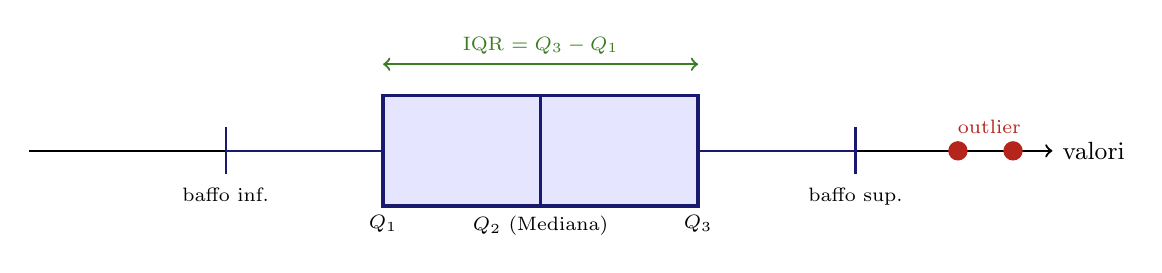
\begin{tikzpicture}[font=\small]
\draw[thick, ->] (-1, 0) -- (12, 0) node[right] {valori};
\draw[fill=blue!10, draw=MidnightBlue, very thick] (3.5, -0.7) rectangle (7.5, 0.7);
\draw[MidnightBlue, very thick] (5.5, -0.7) -- (5.5, 0.7);
\draw[MidnightBlue, thick] (1.5, -0.3) -- (1.5, 0.3);
\draw[MidnightBlue, thick] (9.5, -0.3) -- (9.5, 0.3);
\draw[MidnightBlue, thick] (1.5, 0) -- (3.5, 0);
\draw[MidnightBlue, thick] (7.5, 0) -- (9.5, 0);
\node[below, font=\scriptsize] at (3.5, -0.7) {$Q_1$};
\node[below, font=\scriptsize] at (5.5, -0.7) {$Q_2$ (Mediana)};
\node[below, font=\scriptsize] at (7.5, -0.7) {$Q_3$};
\node[below, font=\scriptsize] at (1.5, -0.35) {baffo inf.};
\node[below, font=\scriptsize] at (9.5, -0.35) {baffo sup.};
\draw[<->, thick, OliveGreen] (3.5, 1.1) -- (7.5, 1.1)
    node[midway, above, font=\scriptsize] {IQR $= Q_3 - Q_1$};
\fill[BrickRed] (10.8, 0) circle (3.5pt);
\fill[BrickRed] (11.5, 0) circle (3.5pt);
\node[above, font=\scriptsize, BrickRed] at (11.2, 0.1) {outlier};
\end{tikzpicture}
\end{center}

La \textbf{regola dei baffi} (regola di Tukey) per identificare gli outlier:
\[
IQR = Q_3 - Q_1
\]
\[
\text{Soglia superiore} = Q_3 + 1{,}5 \times IQR
\qquad
\text{Soglia inferiore} = Q_1 - 1{,}5 \times IQR
\]

I punti che cadono oltre i baffi sono rappresentati come pallini separati e classificati come potenziali anomalie.

\begin{exbox}[EDA pratica -- come impostare \texttt{contamination}]
Se un boxplot mostra che circa il 3\% dei punti cade oltre i baffi, si può impostare \texttt{contamination=0.03} in Isolation Forest come stima iniziale. La scelta finale è una decisione di dominio: quanto costa un falso allarme rispetto a un'anomalia mancata?
\end{exbox}

\section{Sintesi degli algoritmi non supervisionati}

\begin{center}
\renewcommand{\arraystretch}{1.4}
\begin{tabular}{@{} l p{4.2cm} p{5.6cm} @{}}
\toprule
\textbf{Algoritmo} & \textbf{Punto di forza} & \textbf{Uso ideale} \\
\midrule
\textbf{K-Means} & Veloce e semplice & Cluster sferici, $k$ noto \\
\textbf{Mini-Batch K-Means} & Scalabilità estrema & Dataset enormi \\
\textbf{DBSCAN} & Forme arbitrarie, gestisce rumore & Cluster non lineari, densità uniforme \\
\textbf{HDBSCAN} & Densità variabili & Estensione robusta di DBSCAN \\
\textbf{Agglomerative} & Dendrogramma, no $k$ fisso & Tassonomie, biologia \\
\textbf{GMM} & Soft, probabilistico, ellittico & Cluster ellissoidali \\
\textbf{Isolation Forest} & Isolamento rapido, scalabile & Anomaly detection, frodi \\
\textbf{One-Class SVM} & Frontiera non lineare & Novelty detection \\
\textbf{LOF} & Densità locale & Anomalie locali \\
\bottomrule
\end{tabular}
\end{center}

\begin{defbox}[Come scegliere l'algoritmo]
\begin{itemize}
    \item Cluster sferici, $k$ noto, dataset grande: \textbf{K-Means} (o Mini-Batch).
    \item Forme arbitrarie, presenza di rumore: \textbf{DBSCAN / HDBSCAN}.
    \item Cluster ellittici, soft assignment, stima densità: \textbf{GMM}.
    \item Rilevazione anomalie scalabile, alta dimensione: \textbf{Isolation Forest}.
    \item Anomalie locali in bassa dimensione: \textbf{LOF}.
\end{itemize}
Non esiste una ``pallottola d'argento'': la scelta dipende dalla forma dei dati, dalla dimensionalità e dall'obiettivo applicativo.
\end{defbox}